% !TEX root = Technologierecherche.tex
\section{Beladen}
\subsection{Erkennung des Containers}
\textbf {Mit Distanzsensoren und Farbsensoren}
\begin{itemize}
\item Unbekannte Genauigkeit muss getestet werden.
\item Benötigt AD Wandler (Wenn Infrarot- oder Ultraschallsensor)
\item Kein mechanischer Kontakt
\end{itemize}
\begin{figure}[h]
	\centering
	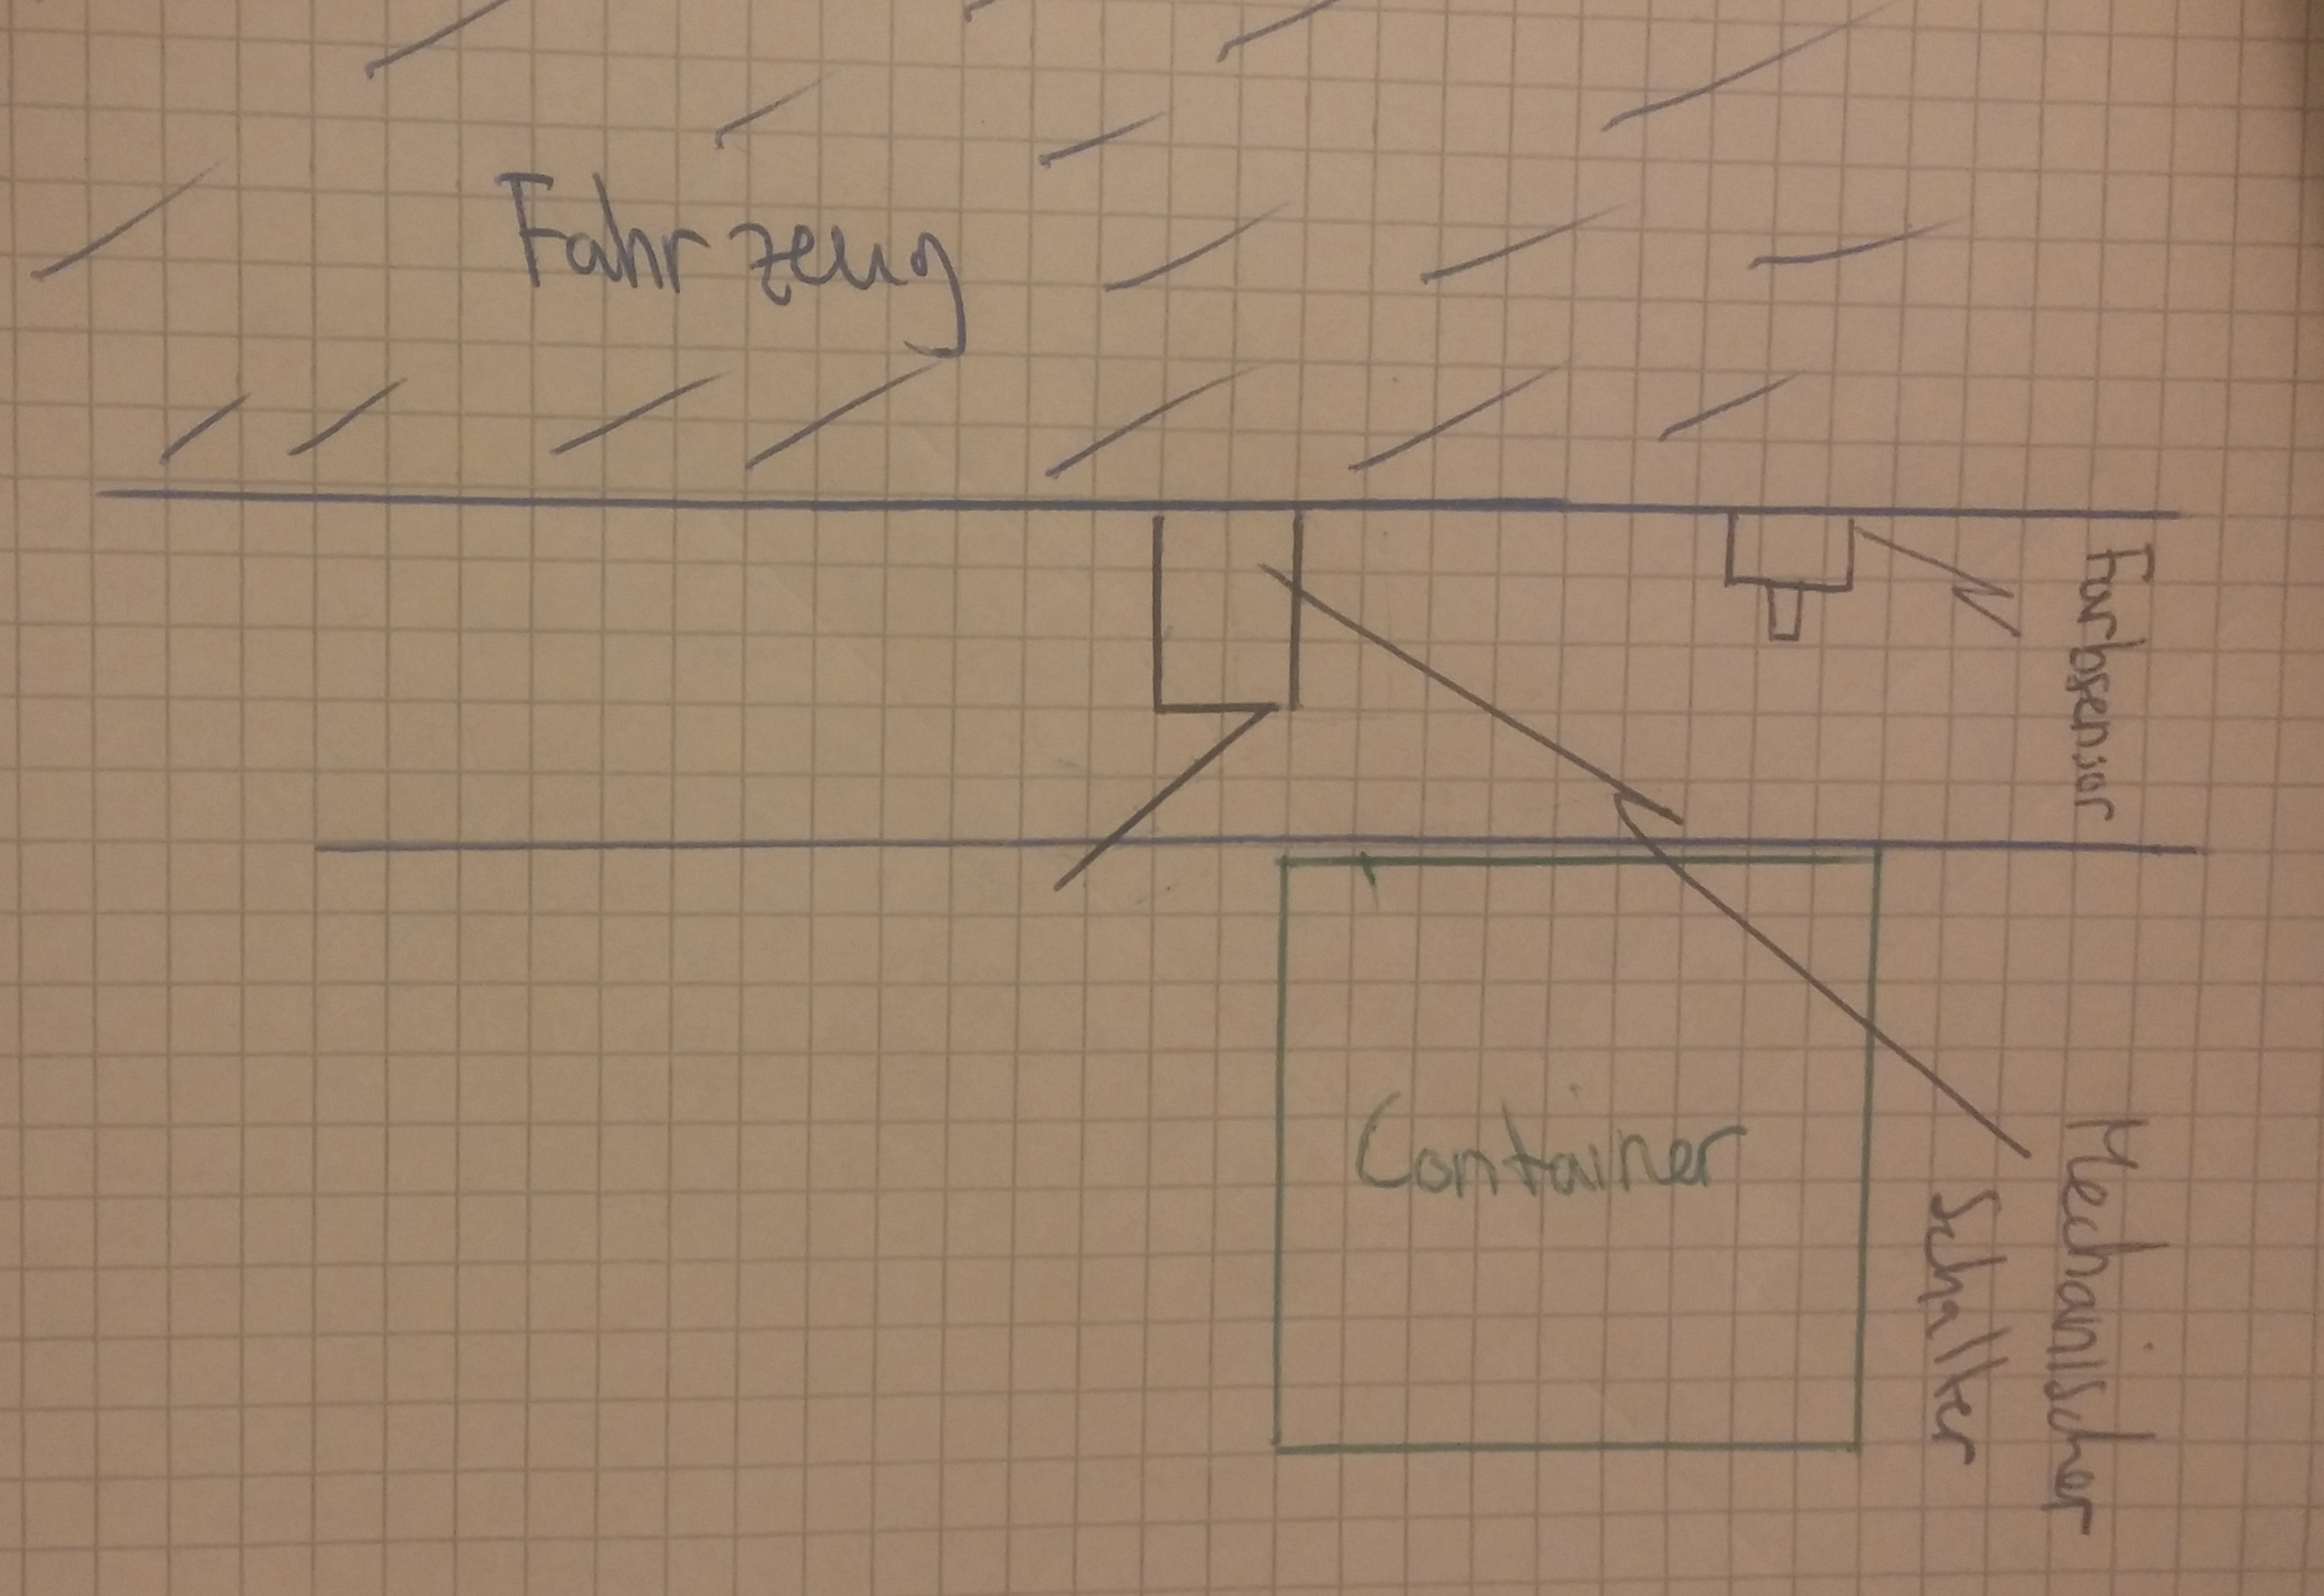
\includegraphics[width=0.5\textwidth]{Images/Containererkennung_1.png}
	\caption{Distanzsensoren an der rechten Seite des Fahrzeugs}
\end{figure}

\textbf {Mechanische Detektion und Farbsensoren}
\begin{itemize}
\item Unbekannte Genauigkeit muss getestet werden.
\item Klarer Wert
\item Mechanischer Kontakt (darf nichts ausser den Container berühren)
\end{itemize}
\begin{figure}[h]
	\centering
	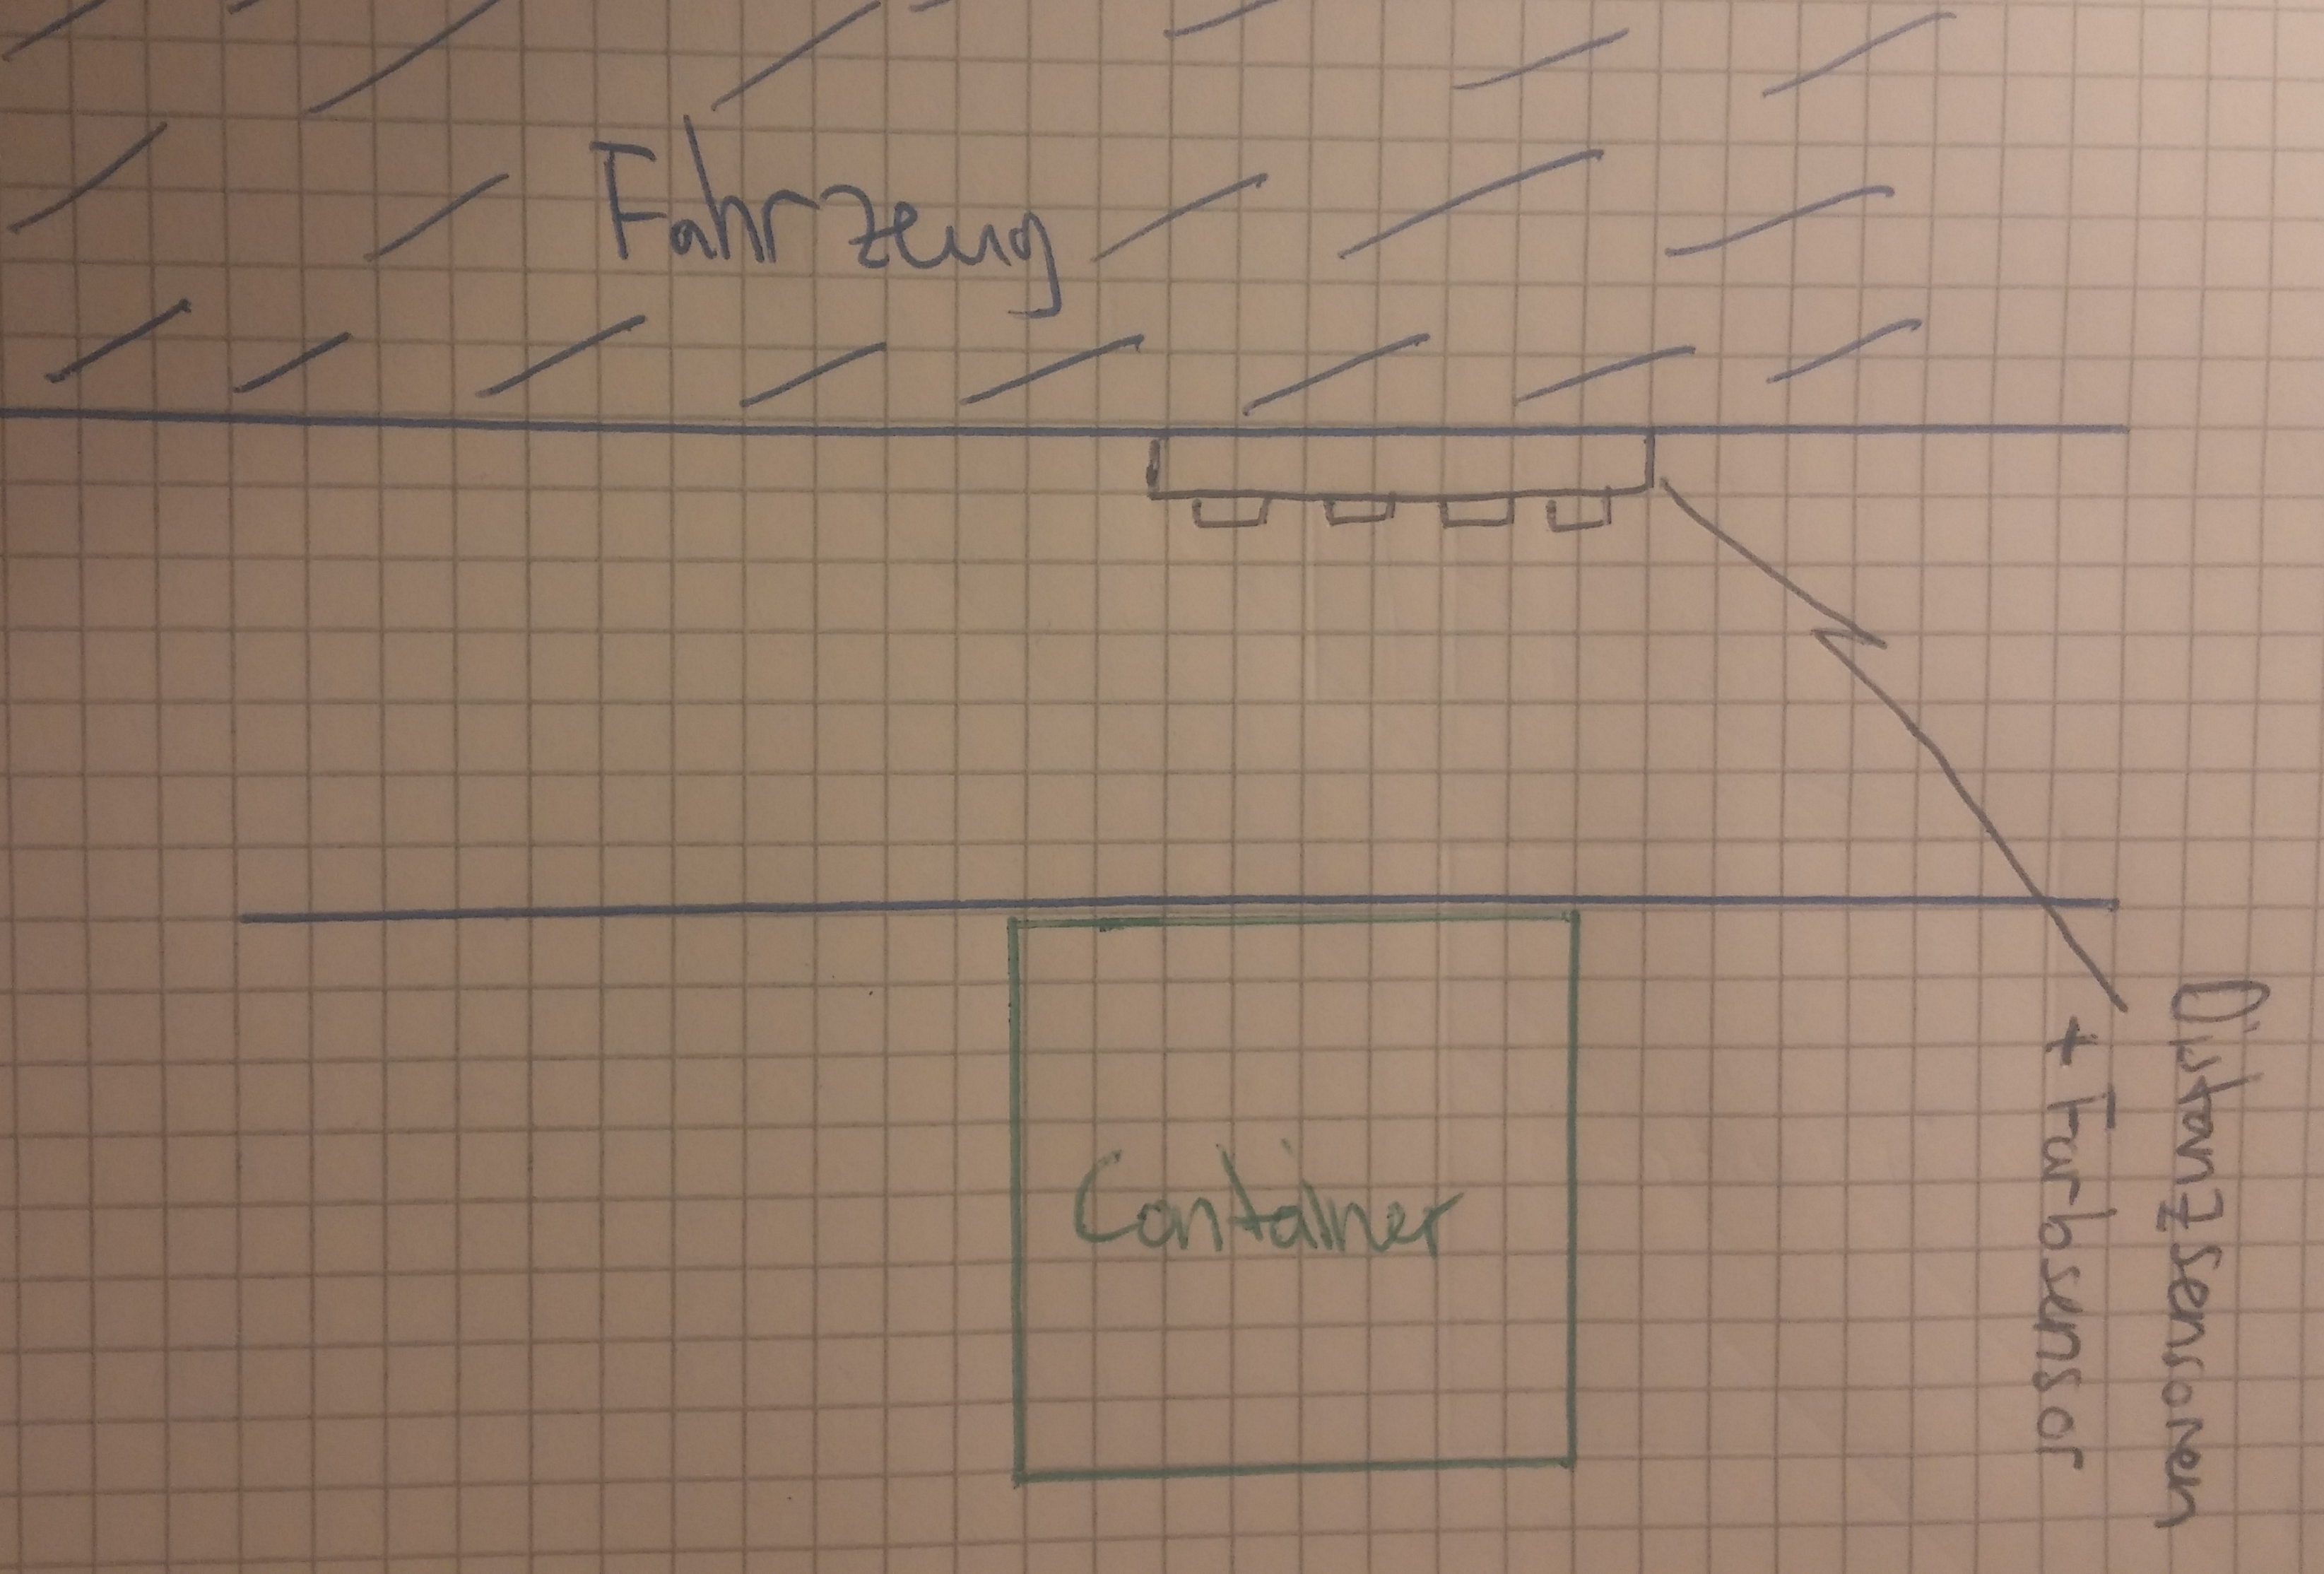
\includegraphics[width=0.5\textwidth]{Images/Containererkennung_2.png}
	\caption{Ein Schalter an der rechten Seite des Fahrzeugs}
\end{figure}

\subsection{Mechanismen die bei Müllfahrzeugen eingesetzt werden}

\begin{itemize}
\item Der Greifer kann senkrecht zur Fahrbahn ausgefahren werden. Zudem ist der Greifer fähig eine Rotation um ca. 135° durchführen. 

Der genaue Mechanismus ist auf youtube (https://www.youtube.com/watch?v=LTUjiLxzDQs)  von 0.08 bis 0.23 ersichtlich.

\item Auf dem selben Video (bei 4:33-4:57) ist ein weiterer Mechanismus zu sehen, der mit einem Knickarm funktioniert. 

\item Bei 5:20-5:50 ist ein sehr einfache und direkte Lösung zu sehen. Es dürfte schwierig sein, diesen Vorgang autonom zu realisieren. 
\end{itemize}